\chapter{Arhitektura i dizajn sustava}
		
Naš sustav se može podijeliti na pet glavnih podsustava koji međusobno komuniciraju:
\begin{description}
	\item[Web preglednik:] Lokalno instalirani program koji omogućuje prikaz sadržaja sa interneta. 
	Pomoću tog programa korisnik može poslati zahtjeve za 
	resursima ili poslati neke podatke web poslužitelju. Web preglednik, 
	nakon što dobije zatražene informacije od web poslužitelja, korisniku prikazuje ssadržaj.

	\item[Web poslužitelj:] Centralni podsustav aplikacije koji obrađuje višestruke zahtjeve korisnika. To 
	može biti zasebno računalo ili samo softver. Komunikaciju s klijentima ostvaruje preko
	HTTP protokola. Web poslužitelj može, na korisnički zahtjev, poslati datoteke ili primiti
	neke podatke koje može spremiti u bazu podataka.

	\item[Baza podataka:] Koristi se za pohranjivanje podataka web apliakcije. Sastavljena je od tablica koje
	predstavljaju entitete s određenim atributima koji su međusobno povezani definiranim
	odnosima. Web aplikacija često komunicira s bazom, povlačeći i davajući podatke bazi.

	\item[Servis za obradu izgovora:] Vanjski servis pomoću kojeg ocjenjujemo izgovor stranih riječi korisnika. Web
	aplikacija komunicira sa servisom preko aplikacijskog sučelja (API).

	\item[Servis za riječi:] Vanjski servis pomoću kojeg administratori lakše stvaraju rječi i, samim time,
	rječnike. Servispreko aplikacijskog sučelja (API) pruža značenja riječi i 
	popratne pomoćne fraze koje olakšavaju proces učenja.
\end{description}


\begin{figure}[h!]
	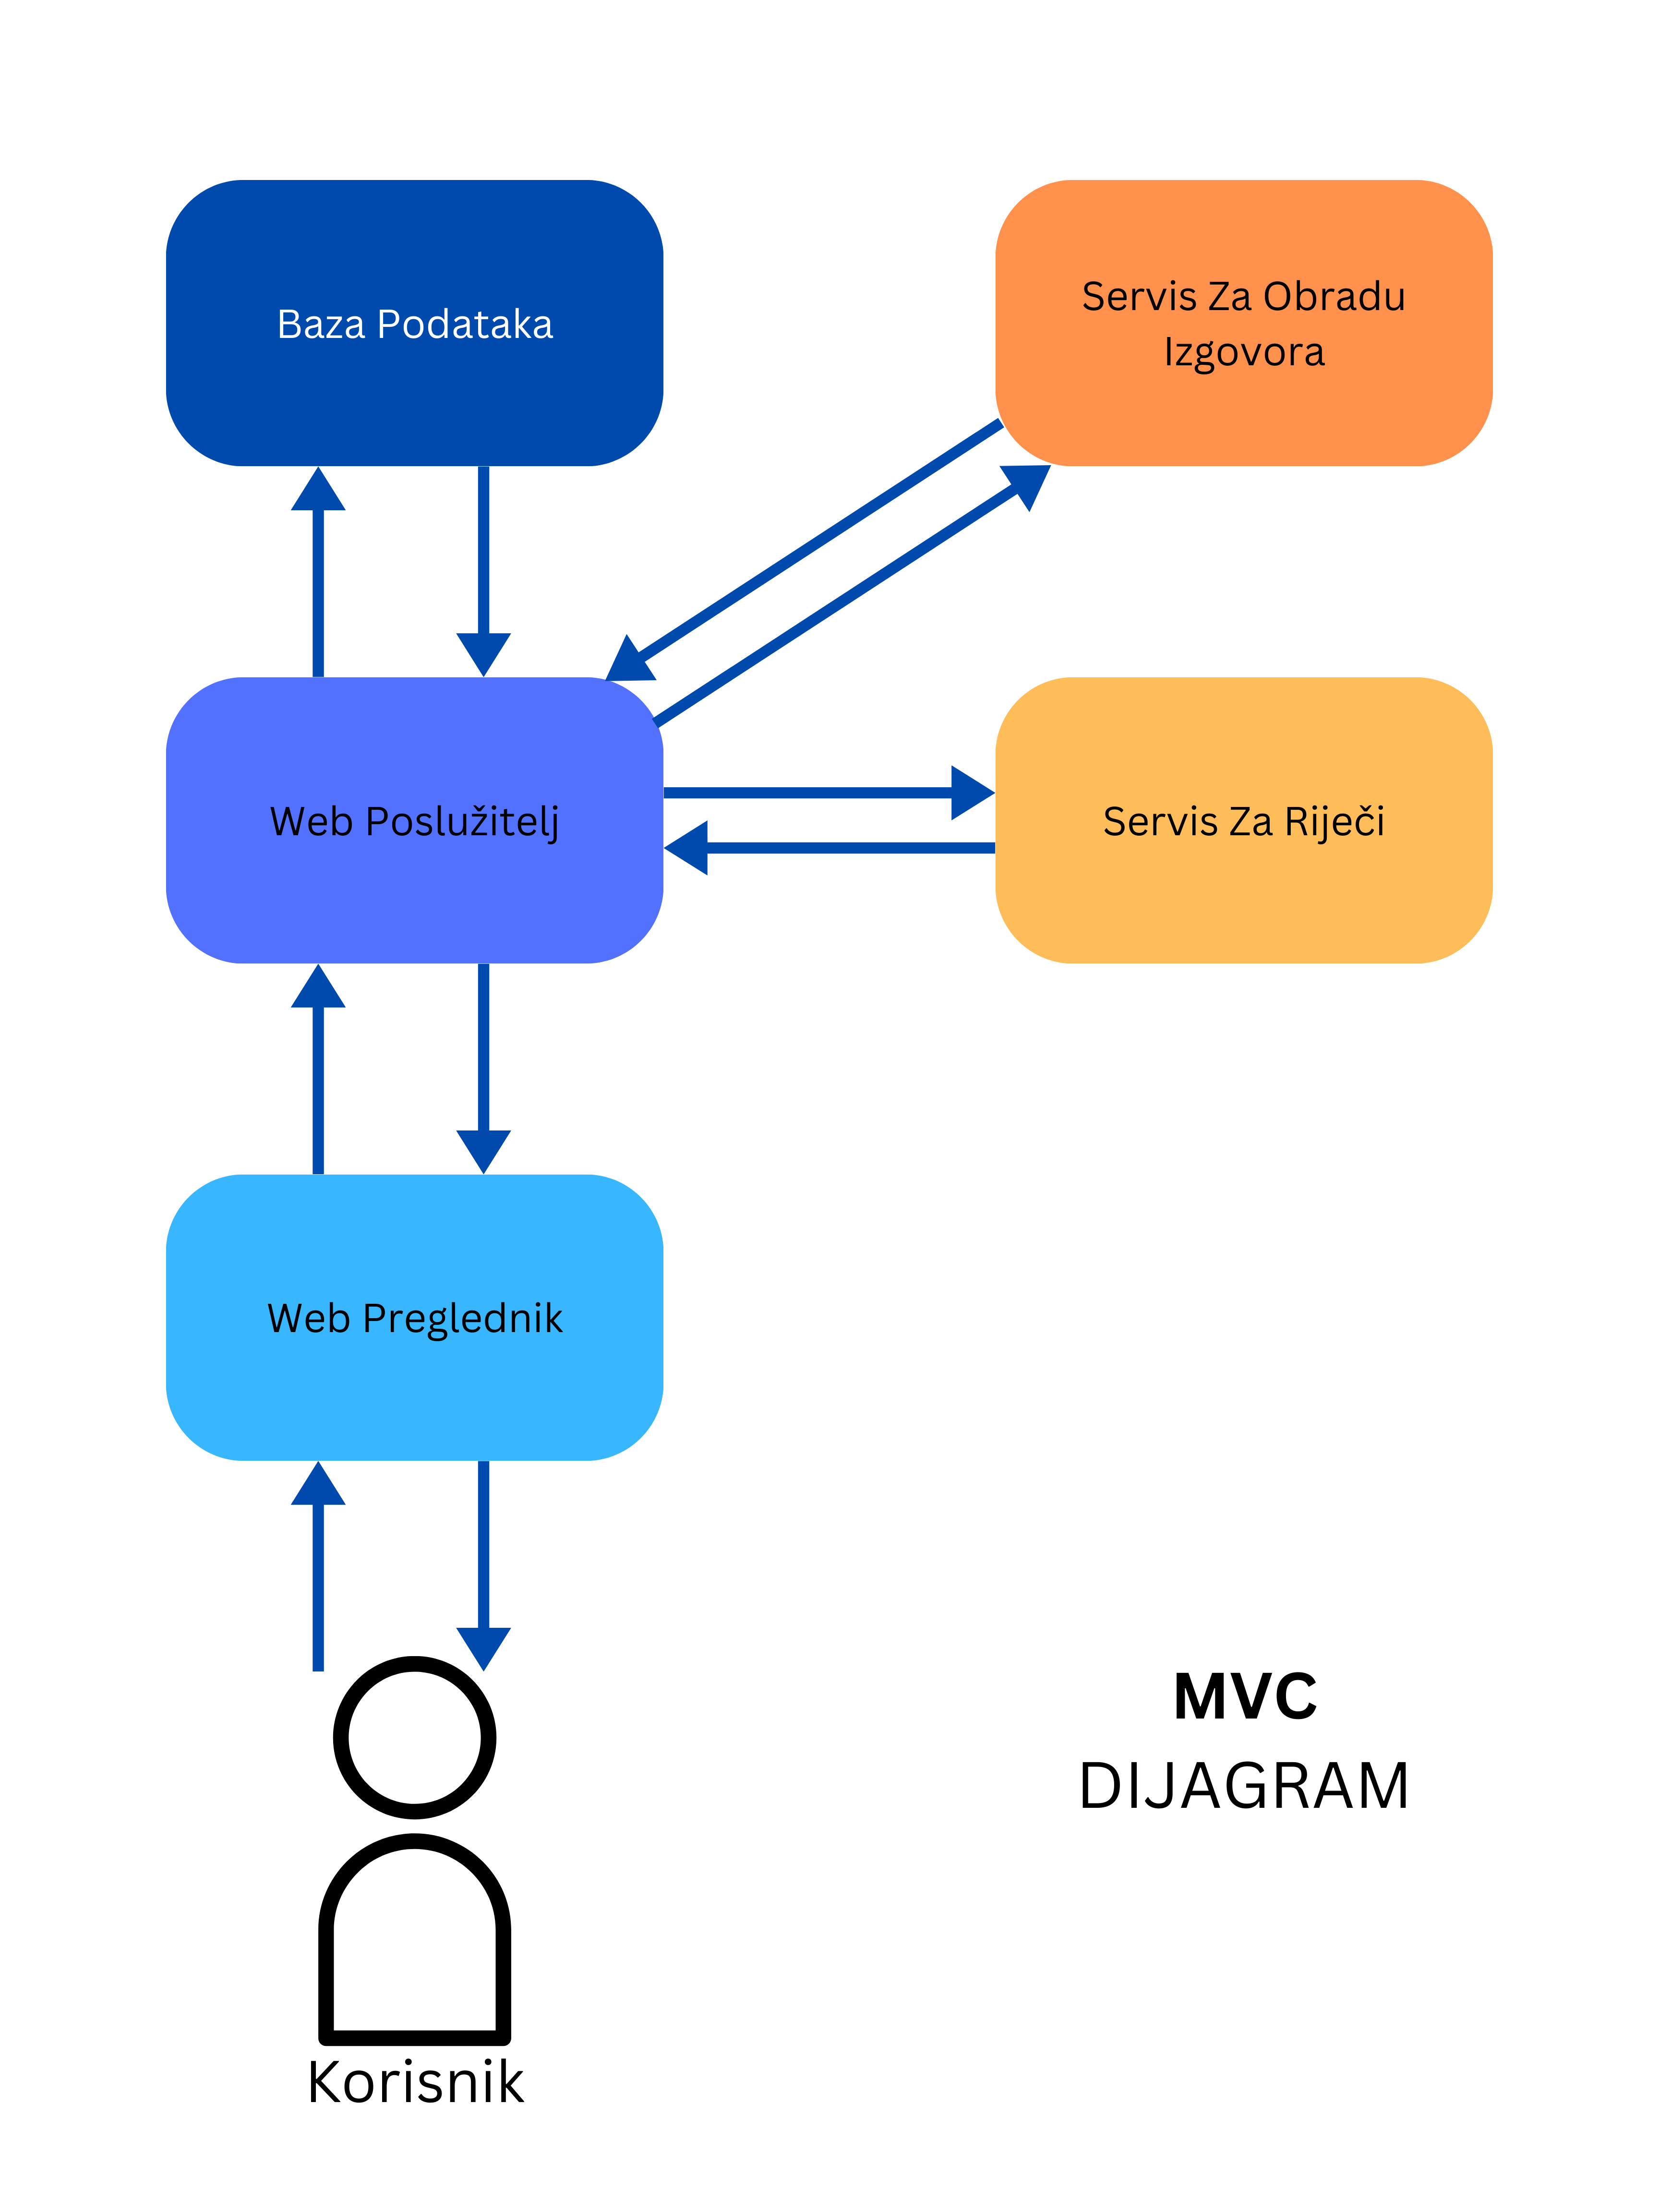
\includegraphics[scale=0.1]{dijagrami/Web Preglednik.png} 
	\centering
	\caption{Shema arhitekture aplikacije}
	\label{fig:mvc-arhitektura}
\end{figure}

\pagebreak

	U izradi aplikaciji koristili smo MVC obrazac dizajna softvera. Elementi tipičnog MVC koncepta su:

	\begin{description}
		\item[\textbf{Model}:] Struktura odgovorna za obradu i upravljanje podacima. 
		\item[\textbf{View}:] Sloj odgovoran za prikazivanje podataka korisnicima.
		\item[\textbf{Controller}:] Sloj koji upravlja logikom aplikacije te surađuje s modelom i pogledom.
	\end{description}


	Backend aplikacije izrađen je u Pythonu korištenjem Flask radnog okvira, dok je za bazu podataka korišten PostgreSQL. Frontend je izrađen u React-u. Također su za funkcionalnost apliakcije korišteni servisi za obradu izgovora i jezičnu provjeru. 
	
		

		

		\pagebreak		
		\section{Baza podataka}

		Naš sustav koristi bazu podataka koja se temelji na relacijskom modelu podataka i koristi tablice (relacije) za organizaciju i pohranu podataka. Entiteti naše baze su: 
		\begin{itemize}
			\item Jezik
			\item Rječnik
			\item Riječ
			\item Korisnik
			\item Fraza
			\item Posuda
		\end{itemize}

			
			
		
			\subsection{Opis tablica}
			

				\textbf{Korisnik} Entitet Korisnik sadrži sve informacije o korisniku. Atributi korisnika su: userId(primarni ključ), ime, prezime, email, lozinka, korisnikStvorenNa, uloga i promijenioLozinku. Korisnik je u \textit{Many-To-One} vezi s tablicom StanjeRiječi.
				
				
				\begin{longtblr}[
					label=none,
					entry=none
					]{
						width = \textwidth,
						colspec={|X[15,l]|X[6, l]|X[20, l]|}, 
						rowhead = 1,
					} %definicija širine tablice, širine stupaca, poravnanje i broja redaka naslova tablice
					\hline \SetCell[c=3]{c}{\textbf{Korisnik}}	 \\ \hline[3pt]
					\SetCell{LightGreen}userId & INT & Identifikacijski ključ korisnika
					  	\\ \hline
					ime	& VARCHAR & Korisnikovo ime  	\\ \hline 
					prezime & VARCHAR & Korisnikovo prezime \\ \hline
					email & VARCHAR & Korisnikov email\\ \hline 
					lozinka & VARCHAR & Korisnikova lozinka \\ \hline
					korisnikStvorenNa & DATETIME & Datum stvaranja računa \\ \hline
					uloga & VARCHAR & Korisnikova uloga (učenik ili admin) \\ \hline
					promijenioLozinku & BOOLEAN & Oznaka je li korisnik promijenio lozinku \\ \hline
					
				\end{longtblr}
				
				\textbf{Rječnik} Entitet Rječnik sadrži sve informacije o rječniku. Njegovi atributi su su: rječnikId(primarni ključ), nazivRječnik, rječnikStvorenNa i jezikId. Rječnik je u \textit{Many-To-One} vezi s tablicom RječnikRiječi te je u \textit{Many-To-One} vezi s entitetom Jezik.


				\begin{longtblr}[
					label=none,
					entry=none
					]{
						width = \textwidth,
						colspec={|X[15,l]|X[6, l]|X[20, l]|}, 
						rowhead = 1,
					} %definicija širine tablice, širine stupaca, poravnanje i broja redaka naslova tablice
					\hline \SetCell[c=3]{c}{\textbf{Rječnik}}	 \\ \hline[3pt]
					\SetCell{LightGreen}rječnikId & INT & Identifikacijski ključ rječnika
					  	\\ \hline
					nazivRječnik	& VARCHAR & Naziv rječnika  	\\ \hline 
					rječnikStvorenNa & DATE & Datum stvaranja rječnika \\ \hline
					\SetCell{LightBlue}
					jezikId & INT & Identifikacijski ključ jezika rječnika\\ \hline 
					
				\end{longtblr}

				\textbf{Riječ} Entitet Riječ sadrži sve informacije o riječi u sustavu. Njeni atributi su su: riječId(primarni ključ), hrvNaziv, straniNaziv, audioPath i jezikId. Entitet Riječ je u \textit{Many-To-One} vezi s entitetom Jezik, u \textit{Many-To-One} vezi s tablicom RiječRječnik, u \textit{One-To-Many} vezi s entitetom Fraza te u \textit{Many-To-One} vezi s tablicom StanjeRiječi.

				\begin{longtblr}[
					label=none,
					entry=none
					]{
						width = \textwidth,
						colspec={|X[15,l]|X[6, l]|X[20, l]|}, 
						rowhead = 1,
					} %definicija širine tablice, širine stupaca, poravnanje i broja redaka naslova tablice
					\hline \SetCell[c=3]{c}{\textbf{Riječ}}	 \\ \hline[3pt]
					\SetCell{LightGreen}riječId & INT & Identifikacijski ključ riječi
					  	\\ \hline
					hrvNaziv & VARCHAR & Naziv riječi na hrvatskom \\ \hline
					straniNaziv	& VARCHAR & Naziv rječi na stranom jeziku 	\\ \hline 
					audioPath	& VARCHAR & Put do audio datoteke s izgovorom riječi  	\\ \hline 
					\SetCell{LightBlue}
					jezikId & INT & Identifikacijski ključ jezika rječnika\\ \hline 
					
				\end{longtblr}

				\textbf{Jezik} Entitet Jezik sadrži sve informacije o nekom jeziku u sustavu. Njegovi atributi su su: jezikId(primarni ključ), nazivJezik i isoOznaka. Entitet Jezik je u \textit{One-To-Many} vezi s entitetom Rječnik te u \textit{One-To-Many} vezi s entitetom Riječ.


				\begin{longtblr}[
					label=none,
					entry=none
					]{
						width = \textwidth,
						colspec={|X[15,l]|X[6, l]|X[20, l]|}, 
						rowhead = 1,
					} %definicija širine tablice, širine stupaca, poravnanje i broja redaka naslova tablice
					\hline \SetCell[c=3]{c}{\textbf{Jezik}}	 \\ \hline[3pt]
					\SetCell{LightGreen}jezikId & INT & Identifikacijski ključ jezika
					  	\\ \hline
					nazivJezik & VARCHAR & Naziv jezika \\ \hline
					isoOznaka	& CHAR(2) & ISO oznaka jezika 	\\ \hline 
					 
					
				\end{longtblr}

				\textbf{Fraza} Entitet Fraza sadrži sve informacije o nekoj frazi u sustavu. Njeni atributi su su: frazaId(primarni ključ), fraza i riječId. Entitet Fraza je u \textit{Many-To-One} vezi s entitetom Riječ.


				\begin{longtblr}[
					label=none,
					entry=none
					]{
						width = \textwidth,
						colspec={|X[15,l]|X[6, l]|X[20, l]|}, 
						rowhead = 1,
					} %definicija širine tablice, širine stupaca, poravnanje i broja redaka naslova tablice
					\hline \SetCell[c=3]{c}{\textbf{Fraza}}	 \\ \hline[3pt]
					\SetCell{LightGreen}frazaId & INT & Identifikacijski ključ fraze
					  	\\ \hline
					fraza & VARCHAR & Puna fraza \\ \hline
					\SetCell{LightBlue}riječId & INT & Identifikacijski ključ riječi iz fraze
					  	\\ \hline
					 
					
				\end{longtblr}

				\textbf{RiječRječnik} Tablica RiječRječnik povezuje sve riječi s pripadnim rječnikom. Njeni atributi su su: riječId(primarni ključ) te rječnikId(primarni ključ). Tablica RiječRječnik je u \textit{One-To-Many} vezi s entitetom Riječ i u \textit{One-To-Many} vezi s entitetom Rječnik.

				\begin{longtblr}[
					label=none,
					entry=none
					]{
						width = \textwidth,
						colspec={|X[15,l]|X[6, l]|X[20, l]|}, 
						rowhead = 1,
					} %definicija širine tablice, širine stupaca, poravnanje i broja redaka naslova tablice
					\hline \SetCell[c=3]{c}{\textbf{RiječRječnik}}	 \\ \hline[3pt]
					\SetCell{LightGreen}riječId & INT & Identifikacijski ključ riječi
					  	\\ \hline
					\SetCell{LightGreen}rječnikId & INT &Identifikacijski ključ rječnika
					\\ \hline
					 
					
				\end{longtblr}


				\textbf{StanjeRiječi} Tablica StanjeRiječi povezuje korisnika s riječima i njima pripadnim "posudama". Njeni atributi su su: userId(primarniKljuč), riječId(primarniKljuč) i posudaId. Tablica StanjeRiječi je u \textit{One-To-Many} vezi s entitetom Riječ, u \textit{One-To-Many} vezi s entitetom Korisnik te u \textit{One-To-One} vezi s entitetom Posuda.

				\begin{longtblr}[
					label=none,
					entry=none
					]{
						width = \textwidth,
						colspec={|X[15,l]|X[6, l]|X[20, l]|}, 
						rowhead = 1,
					} %definicija širine tablice, širine stupaca, poravnanje i broja redaka naslova tablice
					\hline \SetCell[c=3]{c}{\textbf{StanjeRiječi}}	 \\ \hline[3pt]
					\\ \hline[3pt]
					\SetCell{LightGreen}userId & INT & Identifikacijski ključ korisnika
					  	\\ \hline
					\SetCell{LightGreen}riječId & INT & Identifikacijski ključ riječi
					  	\\ \hline
					\SetCell{LightBlue}posudaId & INT & Identifikacijski ključ posude
					  	\\ \hline 
					
				\end{longtblr}

				\textbf{Posuda} Entitet Posuda predstavlja sve posude i njihove intervale. Njeni atributi su su: posudaId(primarni ključ) i interval. Tablica Posuda je u \textit{One-To-One} vezi s tablicom StanjeRiječi.


				\begin{longtblr}[
					label=none,
					entry=none
					]{
						width = \textwidth,
						colspec={|X[15,l]|X[6, l]|X[20, l]|}, 
						rowhead = 1,
					} %definicija širine tablice, širine stupaca, poravnanje i broja redaka naslova tablice
					\hline \SetCell[c=3]{c}{\textbf{Posuda}}	 \\ \hline[3pt]
					\SetCell{LightGreen}posudaId & INT & Identifikacijski ključ posude
					  	\\ \hline
					interval & INT & Interval čekanja do ponovnog pojavljivanja riječi \\ \hline
					
					 
					
				\end{longtblr}


			
			\subsection{Dijagram baze podataka}

				\begin{figure}[H]
					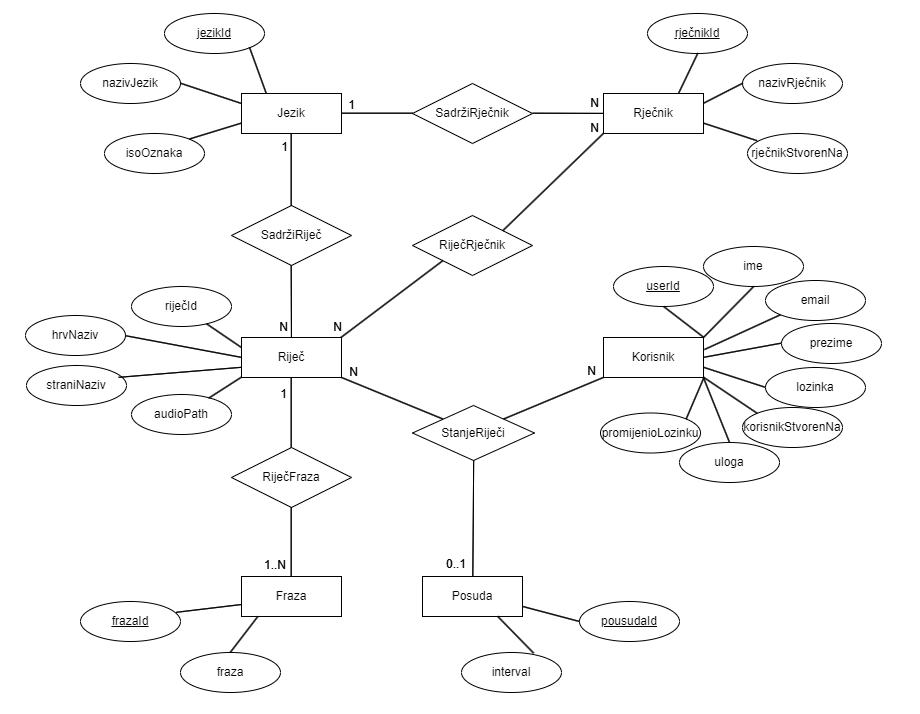
\includegraphics[scale=0.5]{dijagrami/ER_model_BP_3.png}
					\centering
					\caption{ER model baze podataka}
					\label{fig:dijagram_ER-BP}
				\end{figure}

				\begin{figure}[H]
					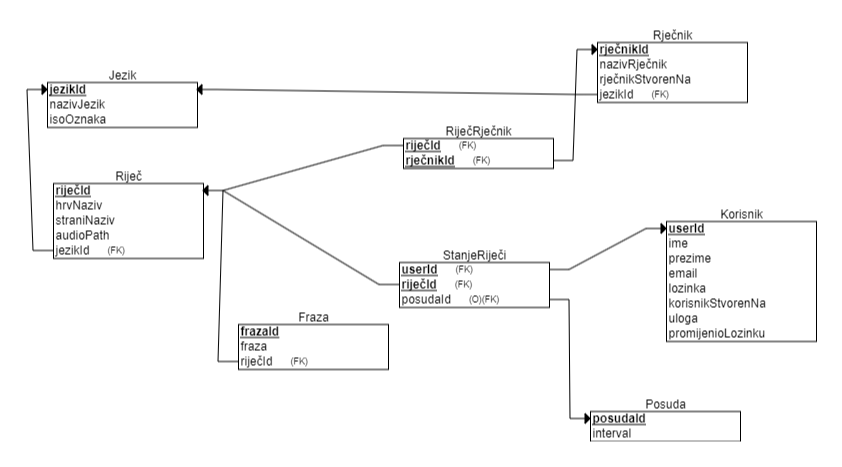
\includegraphics[scale=0.5]{dijagrami/relacijski_model.png}
					\centering
					\caption{Relacijska shema baze podataka}
					\label{fig:dijagram_REL-SH_BP}
				\end{figure}
			
			\eject
			
			
		\section{Dijagram razreda}
		
			\textit{Potrebno je priložiti dijagram razreda s pripadajućim opisom. Zbog preglednosti je moguće dijagram razlomiti na više njih, ali moraju biti grupirani prema sličnim razinama apstrakcije i srodnim funkcionalnostima.}\\
			
			\textbf{\textit{dio 1. revizije}}\\
			
			\textit{Prilikom prve predaje projekta, potrebno je priložiti potpuno razrađen dijagram razreda vezan uz \textbf{generičku funkcionalnost} sustava. Ostale funkcionalnosti trebaju biti idejno razrađene u dijagramu sa sljedećim komponentama: nazivi razreda, nazivi metoda i vrste pristupa metodama (npr. javni, zaštićeni), nazivi atributa razreda, veze i odnosi između razreda.}\\
			
			\textbf{\textit{dio 2. revizije}}\\			
			
			\textit{Prilikom druge predaje projekta dijagram razreda i opisi moraju odgovarati stvarnom stanju implementacije}
			
			
			
			\eject
		
		\section{Dijagram stanja}
			
			
			\textbf{\textit{dio 2. revizije}}\\
			
			\textit{Potrebno je priložiti dijagram stanja i opisati ga. Dovoljan je jedan dijagram stanja koji prikazuje \textbf{značajan dio funkcionalnosti} sustava. Na primjer, stanja korisničkog sučelja i tijek korištenja neke ključne funkcionalnosti jesu značajan dio sustava, a registracija i prijava nisu. }
			
			
			\eject 
		
		\section{Dijagram aktivnosti}
			
			\textbf{\textit{dio 2. revizije}}\\
			
			 \textit{Potrebno je priložiti dijagram aktivnosti s pripadajućim opisom. Dijagram aktivnosti treba prikazivati značajan dio sustava.}
			
			\eject
		\section{Dijagram komponenti}
		
			\textbf{\textit{dio 2. revizije}}\\
		
			 \textit{Potrebno je priložiti dijagram komponenti s pripadajućim opisom. Dijagram komponenti treba prikazivati strukturu cijele aplikacije.}